\documentclass[9pt, oneside]{amsart}   	% use "amsart" instead of "article" for AMSLaTeX format
\usepackage[top=1cm,left=1.2cm, right=1.2cm, bottom=1cm]{geometry}                		% See geometry.pdf to learn the layout options. There are lots.
\geometry{letterpaper}                   		% ... or a4paper or a5paper or ... 
%\geometry{landscape}                		% Activate for rotated page geometry
%\usepackage[parfill]{parskip}    		% Activate to begin paragraphs with an empty line rather than an indent
\usepackage{graphicx}				% Use pdf, png, jpg, or eps§ with pdflatex; use eps in DVI mode
\usepackage{bm}							% TeX will automatically convert eps --> pdf in pdflatex		
\usepackage{amssymb}
\usepackage{amsmath}
\usepackage{subcaption}
\usepackage{float}
\pagenumbering{gobble}
%SetFonts

%SetFonts


\title{}
\author{}
\date{}							% Activate to display a given date or no date

\begin{document}

\section{Learning in discrete graphical models}
Let $(\mathbf{x}_i ,\mathbf{z}_i)_{1, ..., n}$ be an i.i.d sample of observations. $p(z)$ can be written as $p(\mathbf{z}_i|\bm{\pi}) = \prod_{m=1}^{M}\pi_m^{z_{im}}$ and $p(\mathbf{x}_i|\mathbf{z}_i, \bm{\Theta}) = \prod_{m,k}(\theta_{mk})^{z_{im}x_{ik}}$
The log-likelihood of the observations as a function of $\bm{\pi}$ and $\bm{\Theta} = (\theta_{mk})$:

\begin{align*}
	\ell(\bm{\pi}, \bm{\Theta}) &= \sum_{i=1}^n \log p(\mathbf{x}_i, \mathbf{z}_i|\bm{\pi}, \bm{\Theta}) = \sum_{i=1}^n\log p(\mathbf{x}_i|\mathbf{z}_i, \bm{\Theta}) + \sum_{i=1}^n \log p(\mathbf{z}_i|\bm{\pi})
\end{align*}
The maximum likelihood estimator of the right term is given by $\bm{\hat{\pi}} = (\frac{n_1}{n}, \frac{n_0}{n}, ..., \frac{n_M}{n})$ (multinomial distribution and the two terms depend on different parameters). For the left term, with $\mathcal{A}_m = \{i | z_{im}=1\}$ the indexes of the pairs with $z=m$, $n_m = |\mathcal{A}_m|$ and $n_{mk}$ the number of pairs $(x=k, z=m)$: 

\begin{align*}
	\sum\log p(\mathbf{x}_i|\mathbf{z}_i, \bm{\Theta}) = \sum_i\sum_{k,m} z_{im}x_{ik}\log\theta_{mk} = \sum_{m=1}^M \left(\sum_{i\in\mathcal{A}_m}\sum_{k=1}^K x_{ik}\log\theta_{mk}\right) = \sum_{m=1}^M  \sum_{k=1}^Kn_{mk}\log\theta_{mk}
\end{align*}
By analogy with the multinomial distribution maximum likelihood estimator, each term in the sum over $m$ is maximized by $\bm{\hat{\theta}}_m = \left(\frac{n_{mk}}{|\mathcal{A}_m|}\right)_k$, hence $\boxed{\bm{\hat{\Theta}}= \left(\frac{n_{mk}}{n_m}\right)_{km}}$ and $\boxed{\bm{\hat{\pi}} = \left(\frac{n_m}{n}\right)_m}$
\newline

\section{Linear classification - Generative model (LDA) (2.1 (a))}
Let $(\mathbf{x}_i , y_i)_{1, ..., n}$ be an i.i.d sample of observations. 
$$p(\mathbf{x}_i, y_i | \pi, \bm{\bm{\mu}}, \bm{\Sigma}) = p(\mathbf{x}_i|y_i)\cdot p(y_i) = \mathcal{N}(\mathbf{x}_i | \bm{\mu}_1, \bm{\Sigma})^{y_i} \mathcal{N}(\mathbf{x}_i | \bm{\mu}_0, \bm{\Sigma})^{1-y_i}\cdot \pi^{y_i}(1-\pi)^{1-y_i}$$
The log-likelihood as a function of all parameters is
\begin{align*}
	\ell(\pi, \bm{\mu}_1, \bm{\mu}_0, \bm{\Sigma}) = \sum_{i}\left( y_i\log\pi+(1-y_i)\log(1-\pi) \right)+ \sum_i y_i \log\mathcal{N}(\mathbf{x}_i| \bm{\mu}_1, \bm{\Sigma}) + \sum_i (1-y_i) \log\mathcal{N}(\mathbf{x}_i| \bm{\mu}_0, \bm{\Sigma})
\end{align*}
The first sum depends only on $\pi$ and is maximized by $\boxed{\hat{\pi} = n_1/n}$. Since we have for the terms depending on $\bm{\mu}_1$
\begin{align*}
	\sum_i y_i \log\mathcal{N}(\mathbf{x}_i|\bm{\mu}_1, \bm{\Sigma}) = -1/2 \sum_i y_i (\mathbf{x}_i- \bm{\mu}_1)^T\bm{\Sigma}^{-1}(\mathbf{x}_i- \bm{\mu}_1) + const.
\end{align*}
By setting the derivatives with respect to $\bm{\mu}_1$ to 0 and by symmetry for $\bm{\mu}_0$: $\boxed{\hat{\bm{\mu}}_1= (1/n_1)\sum y_i\mathbf{x}_i}$ and $\boxed{\hat{\bm{\mu}}_0 = (1/n_0)\sum (1-y_i)\mathbf{x}_i}$. The terms depending on $\bm{\Sigma}$ are 

\begin{align*}
	-\dfrac{1}{2}\sum_i y_i\left(\log|\bm{\Sigma}| + (\mathbf{x}_i - \bm{\mu}_1)^T\bm{\Sigma}^{-1} (\mathbf{x}_i - \bm{\mu}_1)\right) - \dfrac{1}{2}\sum_i (1-y_i)\left(\log|\bm{\Sigma}| + (\mathbf{x}_i - \bm{\mu}_0)^T\bm{\Sigma}^{-1} (\mathbf{x}_i - \bm{\mu}_0)\right) =\\ -\dfrac{n}{2}\log|\bm{\Sigma}| -\dfrac{n}{2}\text{tr}(\bm{\Sigma}^{-1}\mathbf{S})
\end{align*}
Where $\mathbf{S} = \frac{n_1}{n}\left(\frac{1}{n_1}\sum_{y_i=1} (\mathbf{x}_i-\bm{\mu}_1)(\mathbf{x}_i - \bm{\mu}_1)^T\right) + \frac{n_0}{n}\left(\frac{1}{n_0}\sum_{y_i=0} (\mathbf{x}_i-\bm{\mu}_0)(\mathbf{x}_i - \bm{\mu}_0)^T\right)$ convex sum of the covariances in each class. We can then find that maximum likelihood estimator for $\bm{\Sigma}$ is $\boxed{ \hat{\bm{\Sigma}} = \mathbf{S}}$ by setting the derivatives to 0 in the above expression.
We now study $p(y|\mathbf{x}) \propto p(\mathbf{x}|y)p(y)$
\begin{align*}
	p(y|\mathbf{x}) \propto \pi^y(1-\pi)^{1-y}\mathcal{N}(\mathbf{x}|\mu_1, \bm{\Sigma})^y \mathcal{N}(\mathbf{x}|\mu_0, \bm{\Sigma})^{1-y} \propto \exp\left( y \left(\log\frac{\pi}{1-\pi} + \frac{1}{2}(\mu_0^T\bm{\Sigma}^{-1}\mu_0 -\mu_1^T\bm{\Sigma}^{-1}\mu_1 ) \right) + y(\mu_1-\mu_0)^T\bm{\Sigma}^{-1}X \right)
\end{align*}
Thus, $p(y=k|\mathbf{x}) = \dfrac{\exp(ya+y\mathbf{b}^T\mathbf{x})}{1 + \exp(a+\mathbf{b}^T\mathbf{x} )}$ and $\boxed{p(y=1|\mathbf{x}) = \sigma(a+\mathbf{b}^T\mathbf{x})}$ with $a$ and $\mathbf{b}$ defined in the above formula. It is therefore equivalent to a logistic regression with a closed formula for the coefficients based on the empirical means, covariances and class repartition of the data.
\newline

\section{Linear classification - QDA model (2.5 (a))}
Results are the same as above for $\hat{\pi}$, $\hat{\bm{\mu}}_1$, $\hat{\bm{\mu}}_0$ but $\hat{\bm{\Sigma}}_1$ and $\hat{\bm{\Sigma}}_0$ must be computed separately. The term of the log-likelihood that depends on $\bm{\Sigma}_1$ is 
\begin{align*}
	-\dfrac{1}{2}\sum_i y_i\left(\log|\bm{\Sigma}_1| + (\mathbf{x}_i - \bm{\mu}_1)^T\bm{\Sigma}_1^{-1} (\mathbf{x}_i - \bm{\mu}_1)\right) = -\dfrac{n_1}{2}\log|\bm{\Sigma}_1| -\dfrac{1}{2}\text{tr}\left(\bm{\Sigma}_1^{-1}\sum_{i|y_i=1}(\mathbf{x}_i - \bm{\mu}_1)(\mathbf{x}_i - \bm{\mu}_1)^T\right)
\end{align*}
Hence $\boxed{\hat{\bm{\Sigma}}_1 = \frac{1}{n_1}\sum_{i|y_i=1}(\mathbf{x}_i - \bm{\mu}_1)(\mathbf{x}_i - \bm{\mu}_1)^T}$ and $\boxed{\hat{\bm{\Sigma}}_0 = \frac{1}{n_0}\sum_{i|y_i=0}(\mathbf{x}_i - \bm{\mu}_0)(\mathbf{x}_i - \bm{\mu}_0)^T}$. 

We also have $\boxed{p(y=1|\mathbf{x}) = \sigma\left(a + \mathbf{b}^T\mathbf{x} + \mathbf{x}^T\mathbf{C}\mathbf{x}\right)}$ with $a= \log\frac{\pi}{1-\pi} + \frac{1}{2}(\mu_0^T\bm{\Sigma_0}^{-1}\mu_0 -\mu_1^T\bm{\Sigma_1}^{-1}\mu_1)$, $\mathbf{b}=\mu_1^T\bm{\Sigma_1}^{-1} - \mu_0^T\bm{\Sigma_0}^{-1}$ and $\mathbf{C} = \bm{\Sigma_0}^{-1} - \bm{\Sigma_1}^{-1}$. The model can be interpreted as a logistic regression in the space of the features $(\mathbf{x}_1, \mathbf{x}_2, \mathbf{x}_1\mathbf{x}_2, \mathbf{x}_1^2, \mathbf{x}_2^2)$ with closed formula for the coefficients.

\clearpage
\begin{figure}[t!]
\centering
\begin{subfigure}{.45\textwidth}
  \centering
  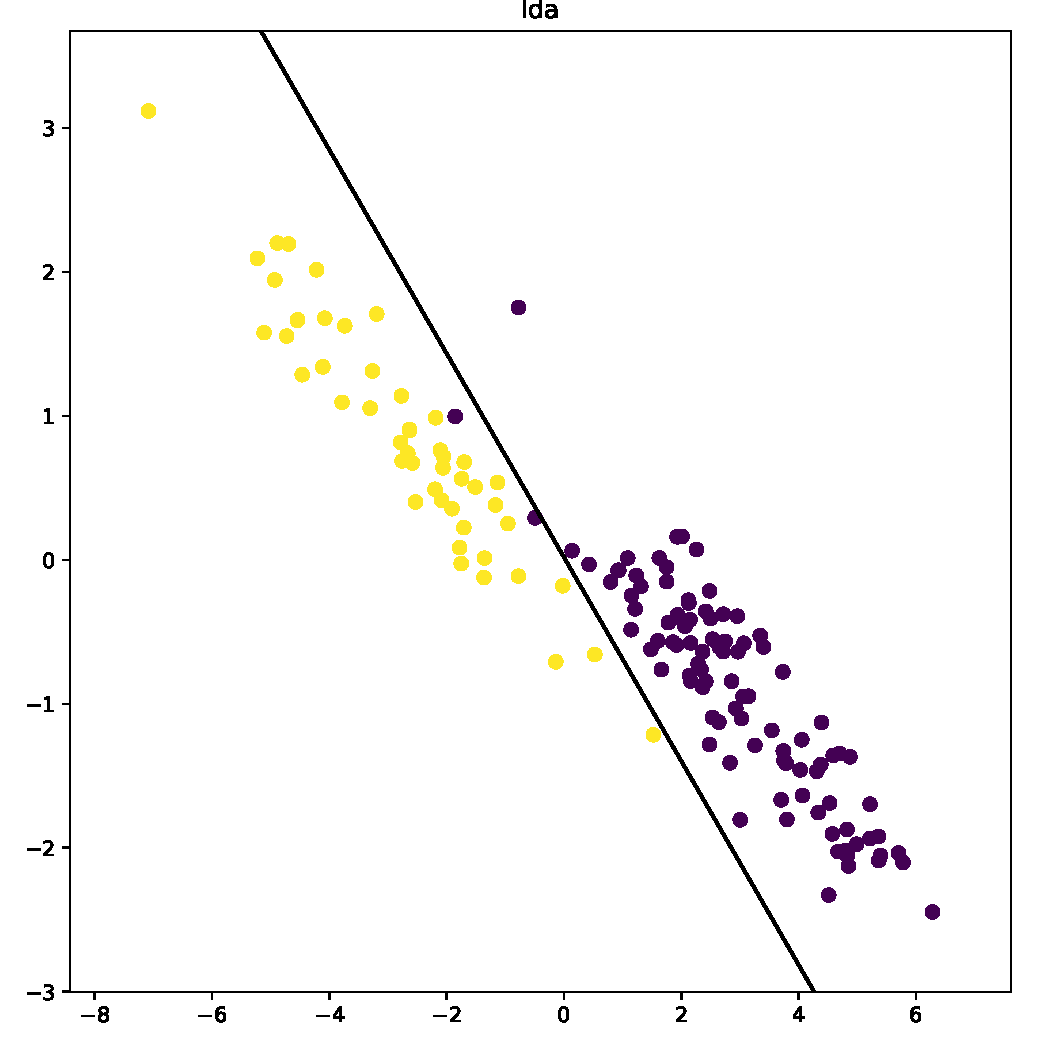
\includegraphics[width=\linewidth]{classificationA_lda.pdf}
 % \caption{Linear Fourier Approximation}
\end{subfigure} \hspace{5pt}
\begin{subfigure}{.45\textwidth}
  \centering
  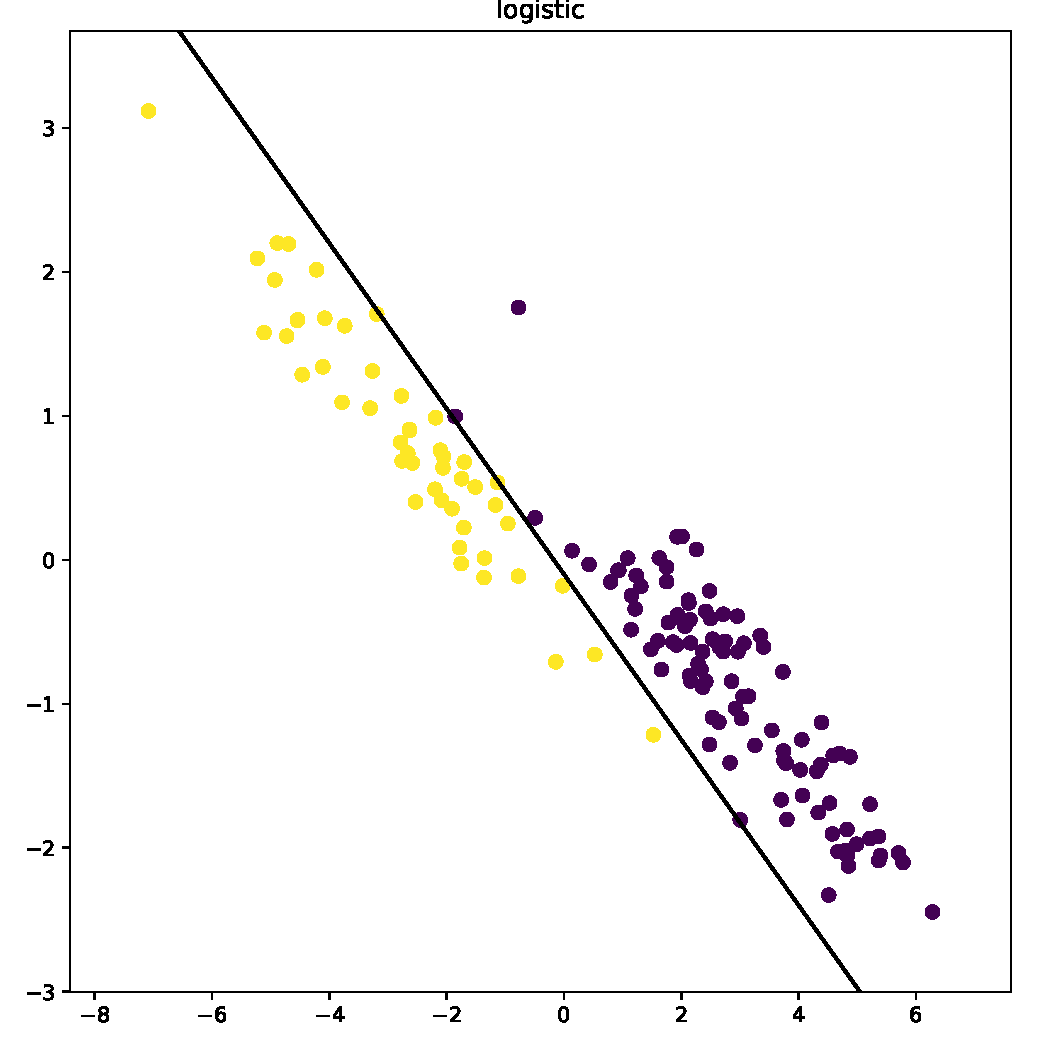
\includegraphics[width=\linewidth]{classificationA_logistic.pdf}
  %\caption{Non-linear Fourier Approximation}
\end{subfigure}
\\[+5pt]
\begin{subfigure}{.45\textwidth}
  \centering
  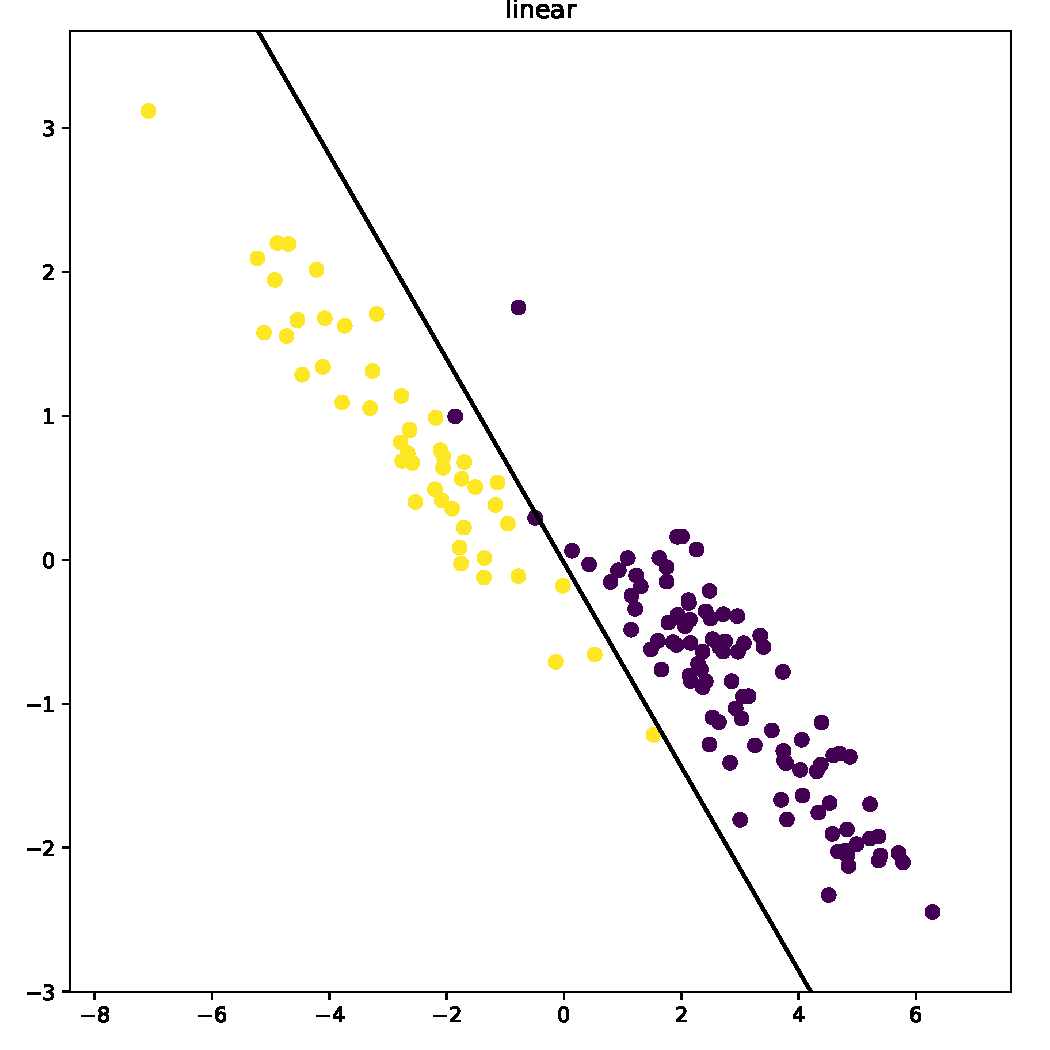
\includegraphics[width=\linewidth]{classificationA_linear.pdf}
  %\caption{Linear Wavelets Approximation}
\end{subfigure} \hspace{5pt}
\begin{subfigure}{.45\textwidth}
  \centering
  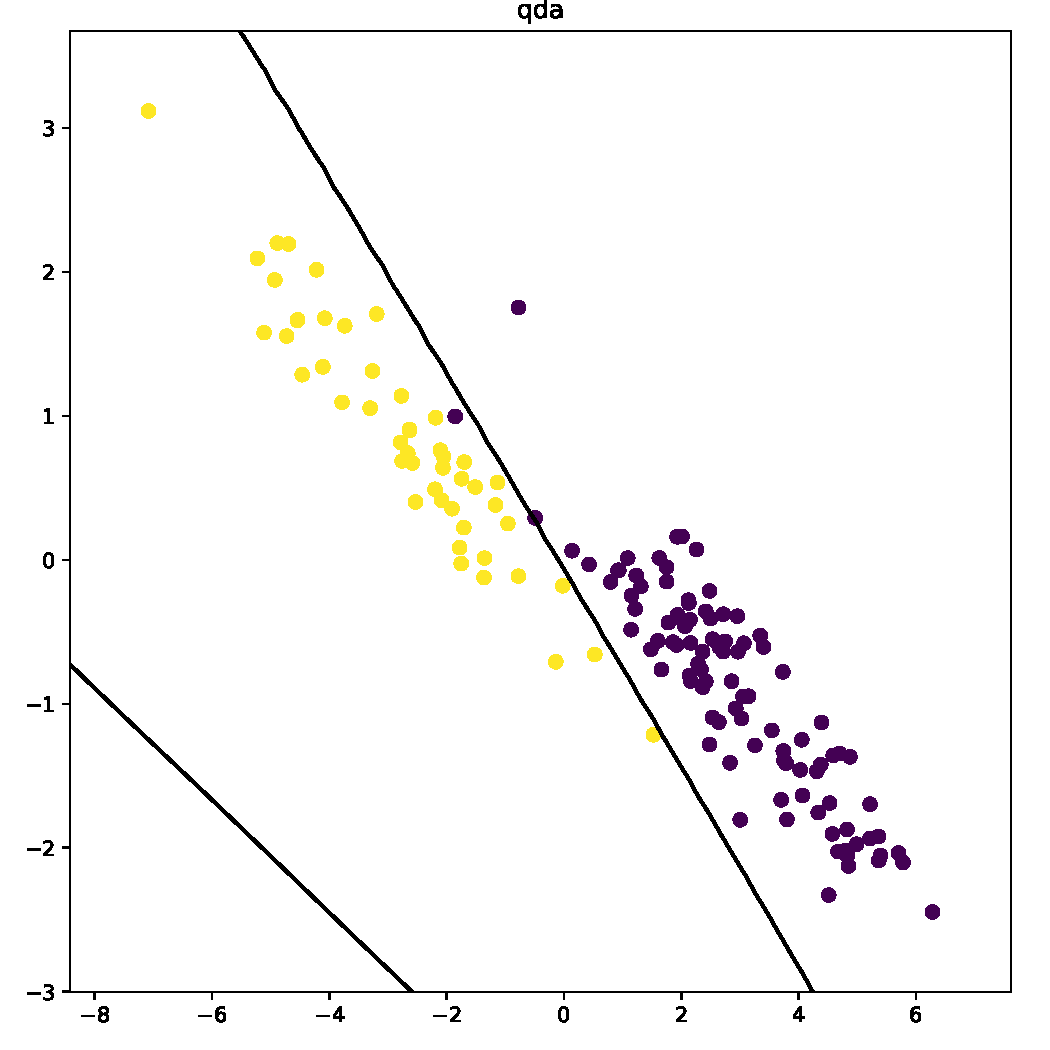
\includegraphics[width=\linewidth]{classificationA_qda.pdf}
  %\caption{Linear Wavelets Approximation}
\end{subfigure}
\end{figure}

\hfill
 \begin{minipage}{.45\textwidth}
  \begin{table}[H]
   \centering
    \begin{tabular}{c|cccc}
    Method & LDA & Logistic & Linear & QDA \\
    \hline
    Train Error & 0.0134 & 0.0000 & 0.0134 & 0.0067 \\
    \hline
    Test Error & 0.0207 & 0.0354 & 0.0207 & 0.0193 \\
    \end{tabular}
\end{table}

 \end{minipage}\hfill
 \begin{minipage}{.45\textwidth}
	Linear Regression and LDA give very similar results, with very close decision boundaries.\\
	The QDA outperforms the other three methods in terms of classification error on the test set.\\
	Since the data is linearly separable, the logistic regression is able to find a separating hyperplane, achieving a 100\% classification score on the train set at the expense of the test error that is higher than for all other methods.
 \end{minipage}\hspace{1cm}


\clearpage
\begin{figure}[t!]
\centering
\begin{subfigure}{.45\textwidth}
  \centering
  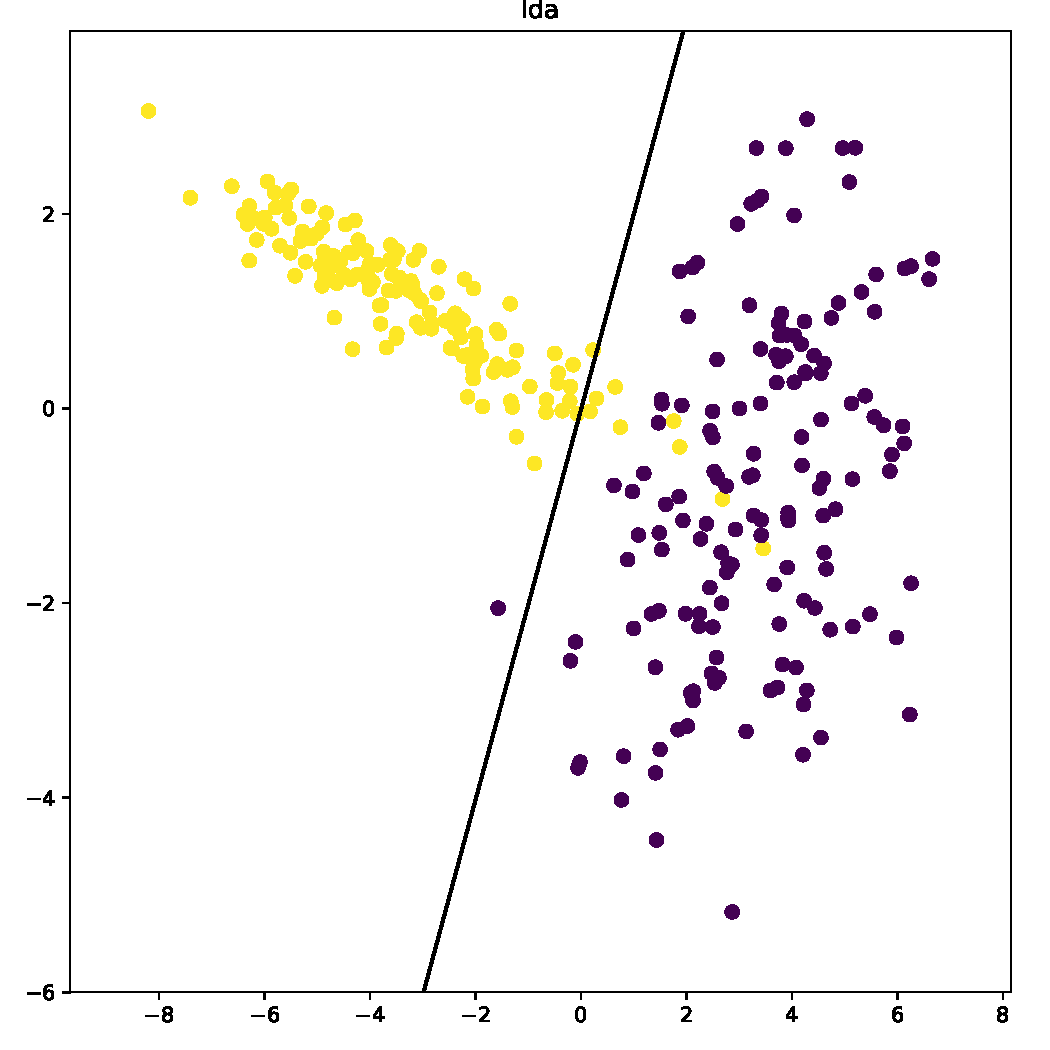
\includegraphics[width=\linewidth]{classificationB_lda.pdf}
 % \caption{Linear Fourier Approximation}
\end{subfigure} \hspace{5pt}
\begin{subfigure}{.45\textwidth}
  \centering
  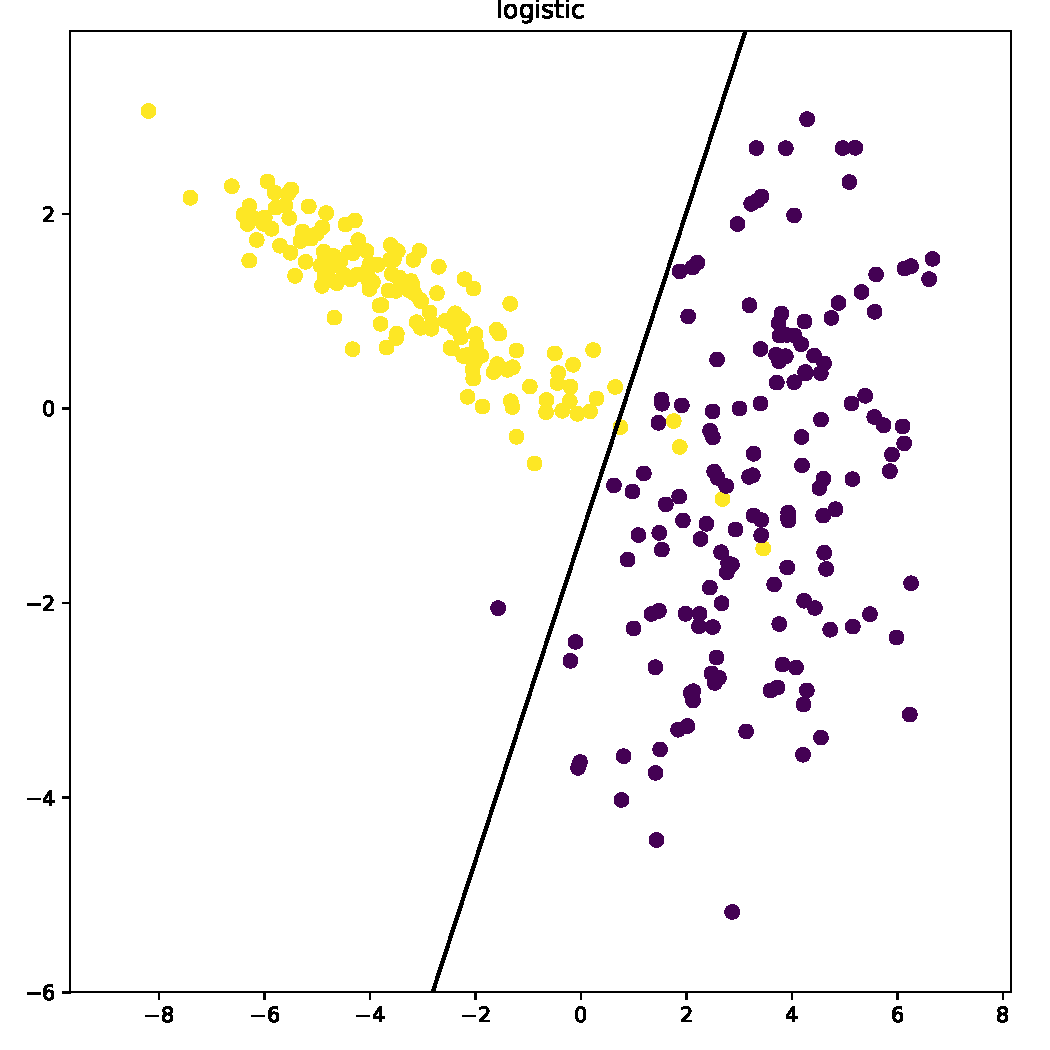
\includegraphics[width=\linewidth]{classificationB_logistic.pdf}
  %\caption{Non-linear Fourier Approximation}
\end{subfigure}
\\[+5pt]
\begin{subfigure}{.45\textwidth}
  \centering
  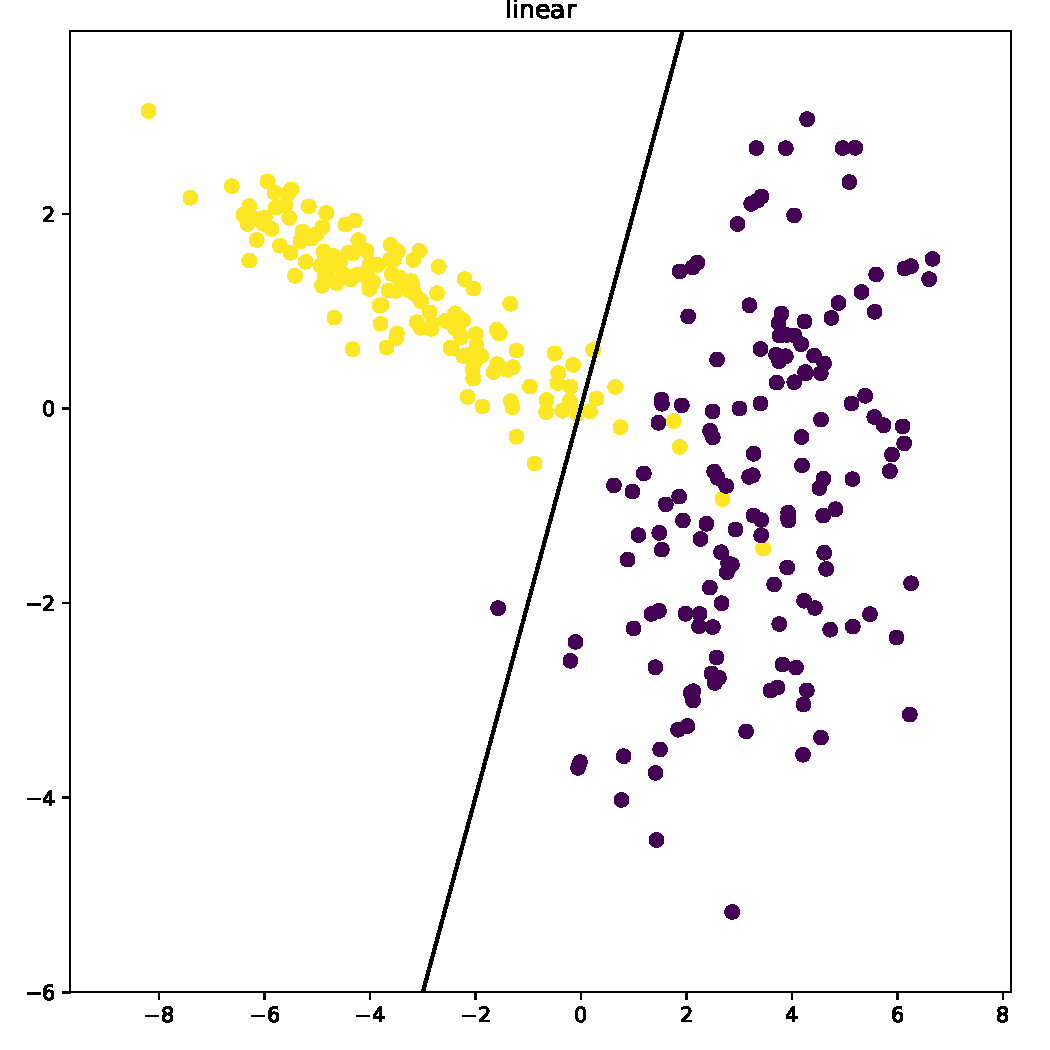
\includegraphics[width=\linewidth]{classificationB_linear.pdf}
  %\caption{Linear Wavelets Approximation}
\end{subfigure} \hspace{5pt}
\begin{subfigure}{.45\textwidth}
  \centering
  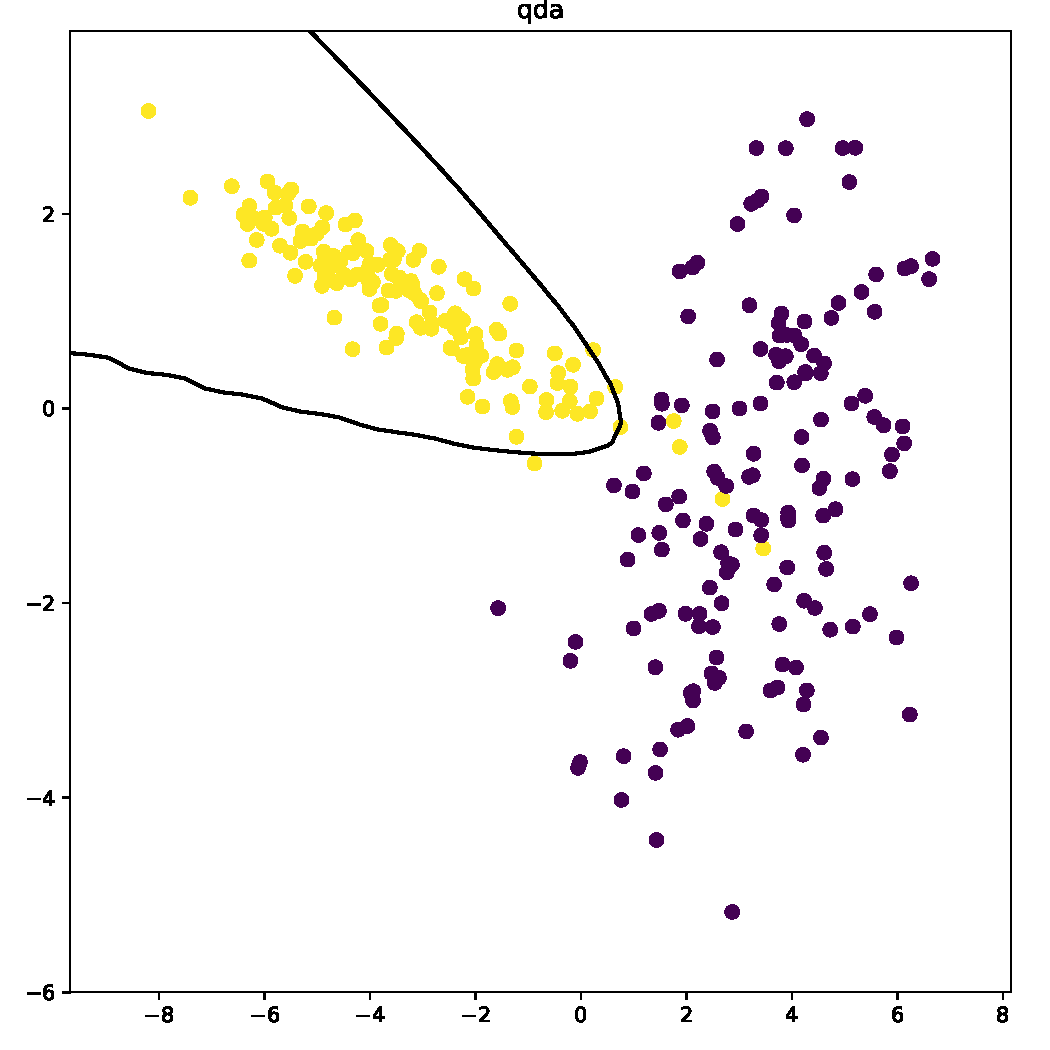
\includegraphics[width=\linewidth]{classificationB_qda.pdf}
  %\caption{Linear Wavelets Approximation}
\end{subfigure}
\end{figure}

\hfill
 \begin{minipage}{.45\textwidth}
  \begin{table}[H]
   \centering
    \begin{tabular}{c|cccc}
    Method & LDA & Logistic & Linear & QDA \\
    \hline
    Train Error & 0.0301 & 0.0201 & 0.0301 & 0.0234 \\
    \hline
    Test Error & 0.0415 & 0.0430 & 0.0415 & 0.0235 \\
    \end{tabular}
\end{table}

 \end{minipage}\hfill
 \begin{minipage}{.45\textwidth}
 The results for linear regression and LDA are again very close. Their decision boundaries don't seem very good compared to the others. For the LDA this is in part due to the fact that the two sets have very different covariances, and assuming they are equal harms the performance of the classification. For the linear regression, the points farther to the left of the yellow set have a much higher least square penalty (linear regression penalizes values far from the objective either above or below) than the points of the blue set, leading to a shift of the decision boundary to the left. 
 
 Logistic regression performs better than LDA and linear regression but still is limited by the linear nature of the boundary it assumes.
 
 The QDA model performs very well because it can cope with the geometric differences between the two sets by letting the covariances being different in the model. 
 \end{minipage}\hspace{1cm}

\clearpage
\begin{figure}[t!]
\centering
\begin{subfigure}{.45\textwidth}
  \centering
  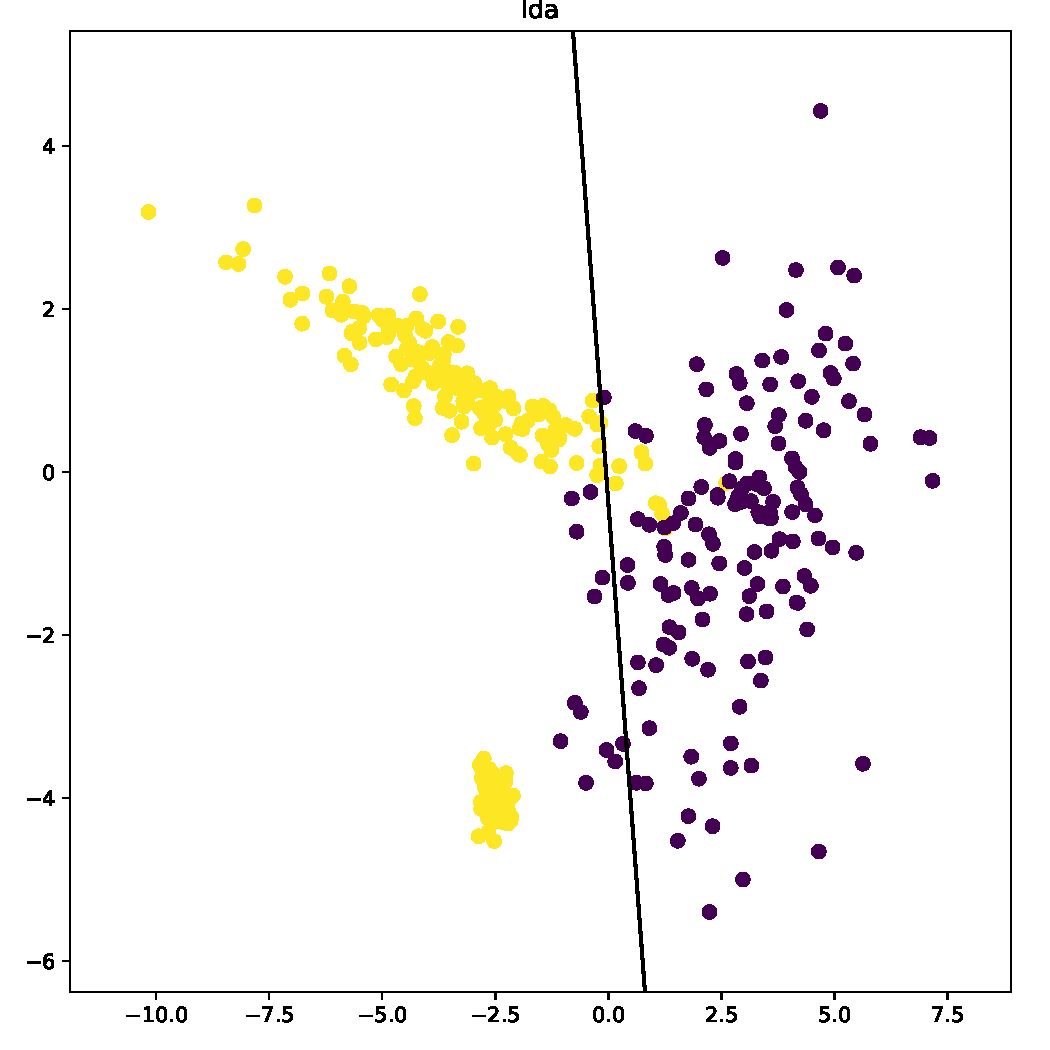
\includegraphics[width=\linewidth]{classificationC_lda.pdf}
 % \caption{Linear Fourier Approximation}
\end{subfigure} \hspace{5pt}
\begin{subfigure}{.45\textwidth}
  \centering
  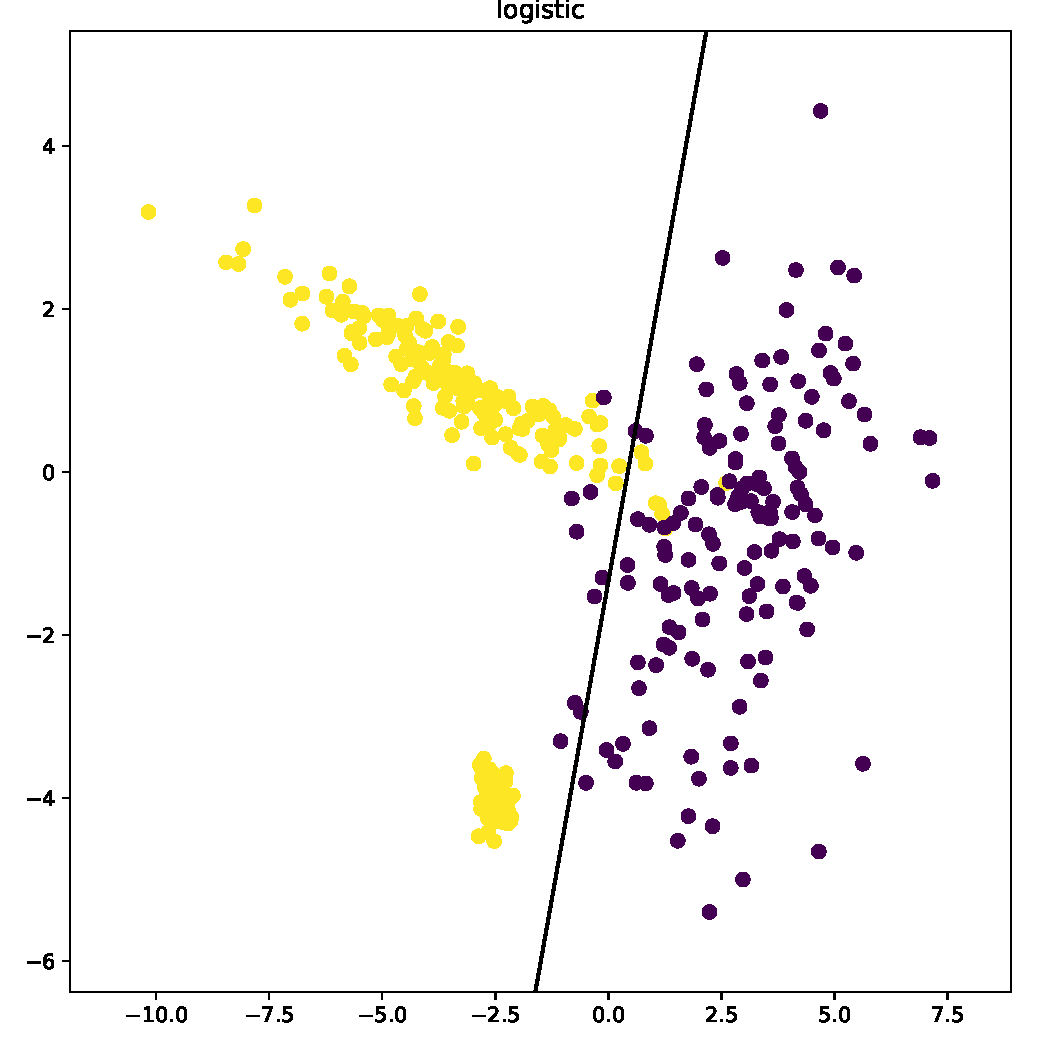
\includegraphics[width=\linewidth]{classificationC_logistic.pdf}
  %\caption{Non-linear Fourier Approximation}
\end{subfigure}
\\[+5pt]
\begin{subfigure}{.45\textwidth}
  \centering
  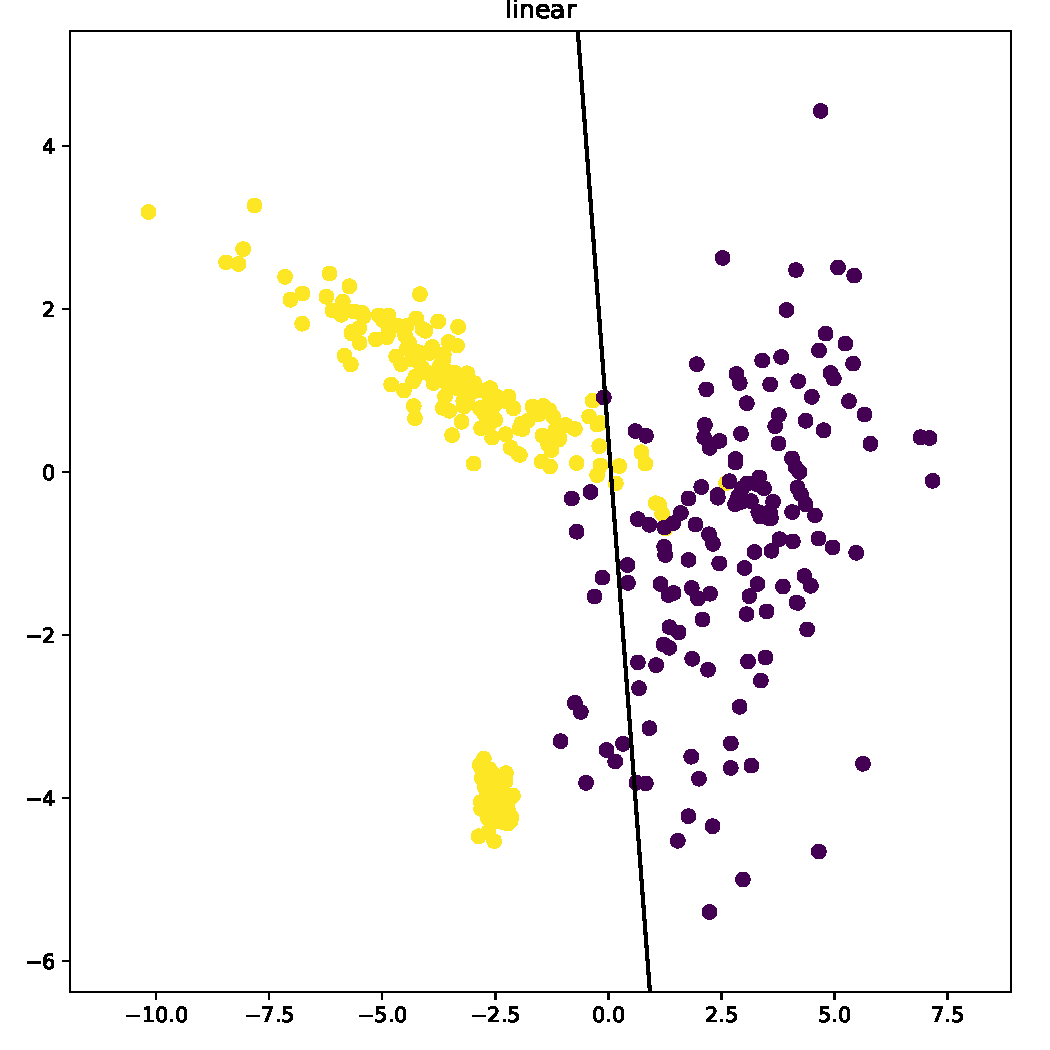
\includegraphics[width=\linewidth]{classificationC_linear.pdf}
  %\caption{Linear Wavelets Approximation}
\end{subfigure} \hspace{5pt}
\begin{subfigure}{.45\textwidth}
  \centering
  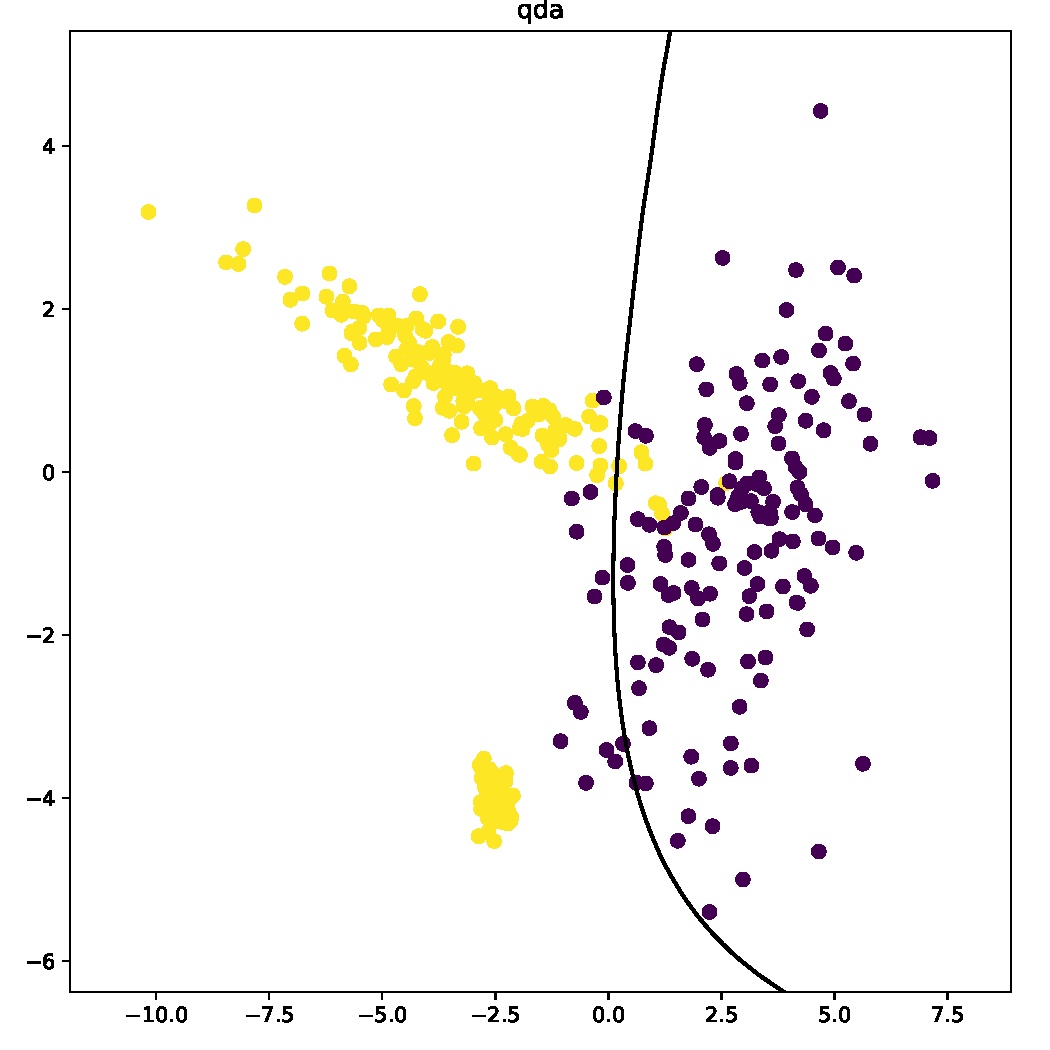
\includegraphics[width=\linewidth]{classificationC_qda.pdf}
  %\caption{Linear Wavelets Approximation}
\end{subfigure}
\end{figure}

\hfill
\begin{minipage}{.45\textwidth}
  \begin{table}[H]
   \centering
    \begin{tabular}{c|cccc}
    Method & LDA & Logistic & Linear & QDA \\
    \hline
    Train Error & 0.0551 & 0.0401 & 0.0551 & 0.0526 \\
    \hline
    Test Error & 0.0420 & 0.0227 & 0.0423 & 0.0403 \\
    \end{tabular}
\end{table}

 \end{minipage}\hfill
 \begin{minipage}{.45\textwidth}
 LDA and logistic regression are affected by the variance and mean shift that the blob of data introduces. The least square penalty moves the frontier such that the blob would be classified closer to 1.  The LDA assumes the data is centered in between the two yellow blobs because it cannot deal with separate sets, which affects its performance negatively.
 
 The logistic regression give better results and is able to handle the blob of data because it is robust to a large number of data points localized in a set and tries to optimize an error function which depends on the quality of classification. 
 
The QDA isn't the most effective model for this data distribution. It is able to handle non linear boundaries that are useful for this kind of complex dataset, but still assumes that data within a class has a Gaussian distribution, which is not the case here.
 \end{minipage}\hspace{1cm}



 \end{document}